\documentclass{apmcmthesis}                                             %
\usepackage{url}                                              
\usepackage{ctex}                                                      
\usepackage{booktabs} % 导言区引入宏包
\usepackage{listings}
\usepackage{xcolor}
\usepackage{hyperref}
\usepackage{amsmath, amssymb, geometry, booktabs}
\geometry{a4paper, margin=1in}
\lstset{
    language=Python,
    basicstyle=\ttfamily\footnotesize,
    keywordstyle=\color{blue},
    stringstyle=\color{red},
    commentstyle=\color{green},
    showstringspaces=false,
    frame=single,
    breaklines=true,
    captionpos=b,
    numbers=left,
    numberstyle=\tiny,
    numbersep=5pt,
    tabsize=4,
    backgroundcolor=\color{gray!10}
}
%%%%%%%%%%%%%%%%%%%%%%%%%%%%%%%%%%%%%%%%%%%%%%%%%%%%%%%%%%%%%%%%%%%%%%%%%
%以上是宏包内容,大家无特殊情况请不要修改%






%%%%%%%%%%%%%%%%%%%%%%%%%%%%%%%%%%%%%%%%%%%%%%%%%%%%%%%%%%%%%%%%%%%%%%%%%
\tihao{A}                            %选题
\baominghao{2516236}                 %参赛编号
\renewcommand{\biaoti}{Image Enhancement Model Based on Deep Learning}
\begin{document}
\pagestyle{frontmatterstyle}
%%%%%%%%%%%%%%%%%%%%%%%%%%%%%%%%%%%%%%%%%%%%%%%%%%%%%%%%%%%%%%%%%%%%%%%%%
%以上填写你的比赛相关信息,你的队伍控制号,你的选题





%%%%%%%%%%%%%%%%%%%%%%%%%%%%%%%%%%%%%%%%%%%%%%%%%%%%%%%%%%%%%%%%%%%%%%%%%
\begin{abstract}
    section*{Abstract}
    %%%%%%%%%%正文
    This study proposes single-task and comprehensive enhancement models for underwater image processing, using deep learning to improve performance across different degradation types.
    \textbf{For Problem 1}, the objective is to classify underwater images based on degradation characteristics using a deep convolutional neural network (CNN). Firstly, the collected data undergoes preprocessing, including image resizing, normalization, and data augmentation. Then, ResNet50 is used as the backbone, combined with a color attention module and a blur detection module to enhance feature extraction. Next, the extracted features are fused through an integration module to generate comprehensive representations. Finally, the fused features are classified into categories such as color shift;low illumination;blur or clear and the results are recorded in an Excel file.
    \textbf{For Problem 2}, the objective is to classify underwater images based on degradation. 
    \textbf{For Problem 3}, the objective is to classify underwater images based on degradation. 
    \textbf{For Problem 4}, the objective is to classify underwater images based on degradation.
    In conclusion, this study establishes a deep learning framework for underwater image enhancement, demonstrating its effectiveness and providing insights for future applications.
    %%%%%%%%%%正文
    %%%%%%%%%%关键词
    \keywords{Underwater Image Processing\quad Deep Learning\quad Image Enhancement\quad GAN}
    %%%%%%%%%%关键词
\end{abstract}
%%%%%%%%%%%%%%%%%%%%%%%%%%%%%%%%%%%%%%%%%%%%%%%%%%%%%%%%%%%%%%%%%%%%%%%%%
%以上的摘要模板只需要修改正文和关键词部分,其他的无需改动




%%%%%%%%%%%%%%%%%%%%%%%%%%%%%%%%%%%%%%%%%%%%%%%%%%%%%%%%%%%%%%%%%%%%%%%%%
\newpage %从新的一页开始
%目录
\tableofcontents
\newpage
\pagestyle{mainmatterstyle}
\setcounter{page}{1}
%%%%%%%%%%%%%%%%%%%%%%%%%%%%%%%%%%%%%%%%%%%%%%%%%%%%%%%%%%%%%%%%%%%%%%%%%
%以上部分用于生成文章的目录页


























%1
%%%%%%%%%%%%%%%%%%%%%%%%%%%%%%%%%%%%%%%%%%%%%%%%%%%%%%%%%%%%%%%%%%%%%%%%%
\section{Introduction}

%1-1
%%%%%%%%%%%%%%%%%%%%%%%%%%%%%%%%%%%%%%%%%%%%%%%%%%%%%%%%%%%%%%%%%%%%%%%%%
\subsection{Background}

这里请写问题的背景,引出研究的目的

%1-2
%%%%%%%%%%%%%%%%%%%%%%%%%%%%%%%%%%%%%%%%%%%%%%%%%%%%%%%%%%%%%%%%%%%%%%%%%
\subsection{Literature Review}

这里请写关于本题的整个研究现状,建议从国内外角度去分析

%1-3
%%%%%%%%%%%%%%%%%%%%%%%%%%%%%%%%%%%%%%%%%%%%%%%%%%%%%%%%%%%%%%%%%%%%%%%%%
\subsection{The Description of the Problem}

以简洁的语言将问题的每一个问重新说一点,如下面的案例所示

\textbf{1. Classification and Analysis of Underwater Image Degradation:}
Utilize statistical methods to classify underwater images, identify the types of degradation, and record the classification basis.

%1-4
%%%%%%%%%%%%%%%%%%%%%%%%%%%%%%%%%%%%%%%%%%%%%%%%%%%%%%%%%%%%%%%%%%%%%%%%%
\subsection{Our work}

这里以总述的口吻写出整个文章的安排,比如说第一问干什么,怎么干,然后第二问、第三问等等。并且要点出问与问之间的协调关系。先文字+流程图,如下案例所示。

This paper proposes a systematic scheme for underwater image degradation in complex scenes. Firstly, the underwater image data is statistically analyzed, and the main degradation types such as color shift, low light and blur are identified and classified by histogram, brightness distribution, edge detection, etc., for the subsequent data support. The detailed process is shown in Figure 1.
\begin{figure}[!th]
    \centering
    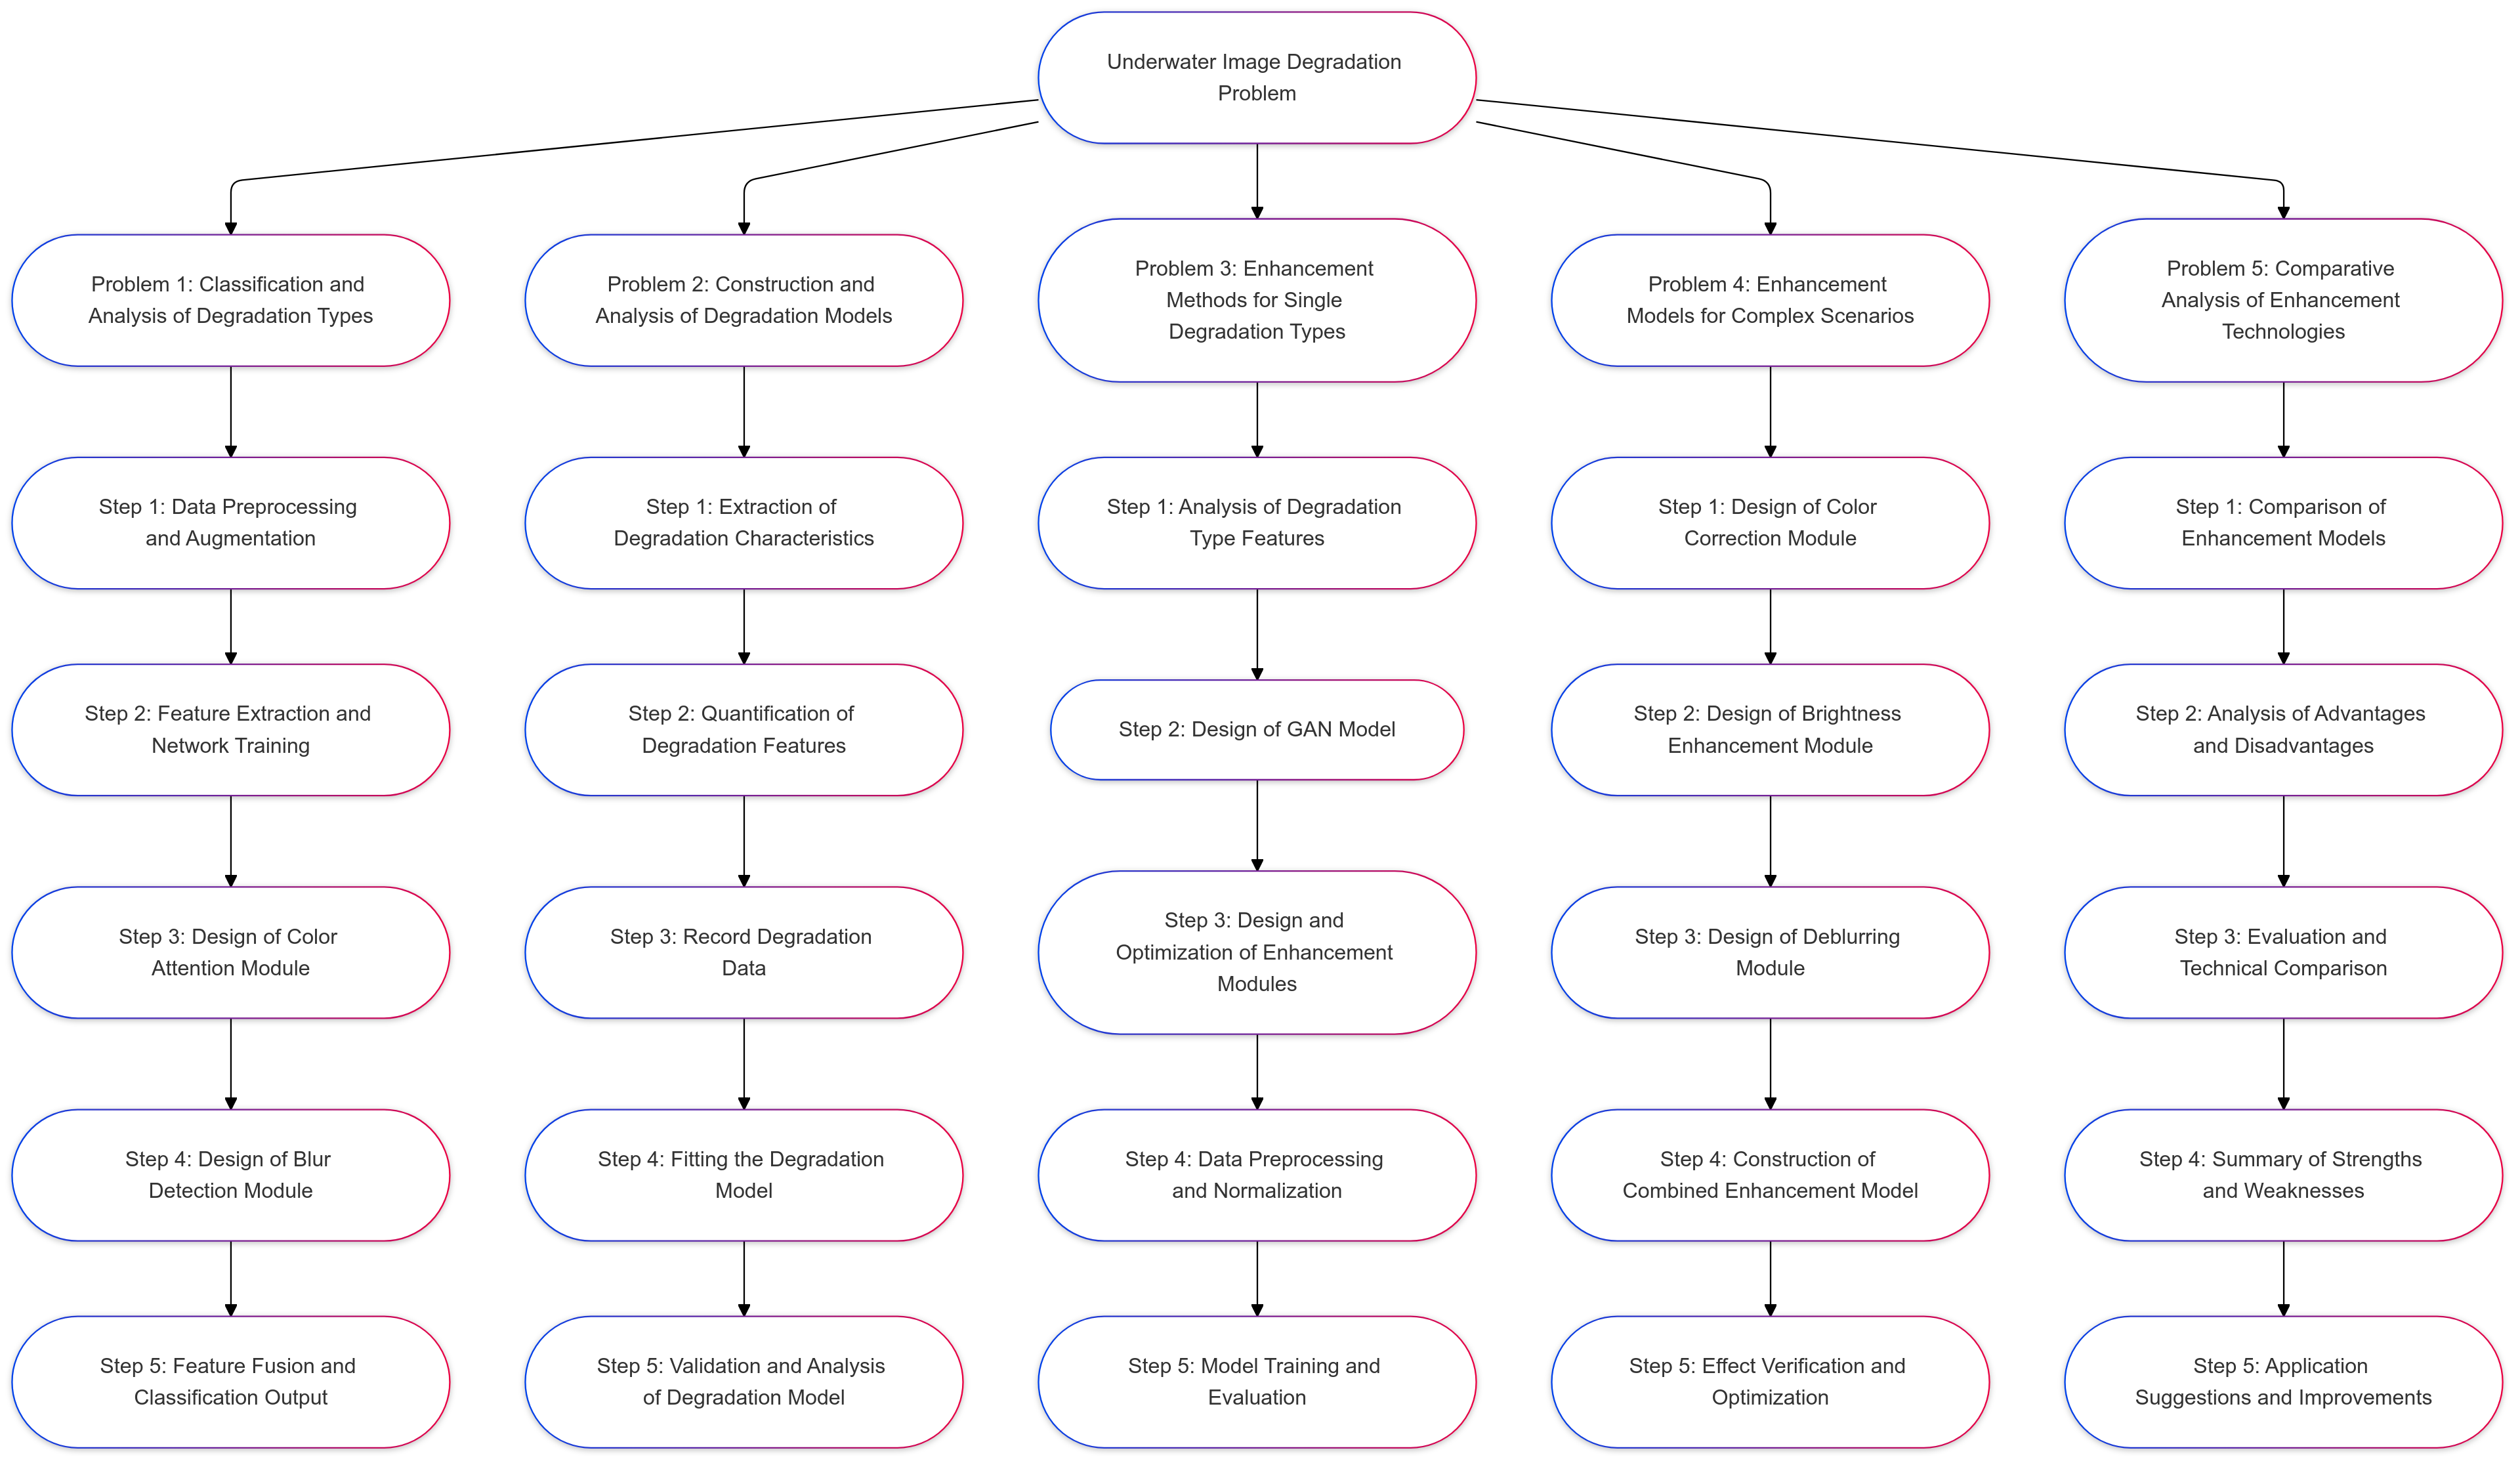
\includegraphics[width=\textwidth]{网络-总体流程图-2024-11-24-081146.png}
    \caption{General flow chart}
    \label{fig:enter-label}
\end{figure}
%%%%%%%%%%%%%%%%%%%%%%%%%%%%%%%%%%%%%%%%%%%%%%%%%%%%%%%%%%%%%%%%%%%%%%%%%
%%%%%%%%%%%%%%%%%%%%%%%%%%%%%%%%%%%%%%%%%%%%%%%%%%%%%%%%%%%%%%%%%%%%%%%%%
%%%%%%%%%%%%%%%%%%%%%%%%%%%%%%%%%%%%%%%%%%%%%%%%%%%%%%%%%%%%%%%%%%%%%%%%%
%%%%%%%%%%%%%%%%%%%%%%%%%%%%%%%%%%%%%%%%%%%%%%%%%%%%%%%%%%%%%%%%%%%%%%%%%
%%%%%%%%%%%%%%%%%%%%%%%%%%%%%%%%%%%%%%%%%%%%%%%%%%%%%%%%%%%%%%%%%%%%%%%%%












\newpage
%2
%%%%%%%%%%%%%%%%%%%%%%%%%%%%%%%%%%%%%%%%%%%%%%%%%%%%%%%%%%%%%%%%%%%%%%%%%
\section{Assumptions}

这里写求解问题需要的一些理论假设,如下面案例所示。

\textbf{Assumption 1:} The light attenuation and scattering in the underwater environment adhere to the Jaffe-McGlamery imaging model, where the propagation of light follows an exponential decay law.





%3
%%%%%%%%%%%%%%%%%%%%%%%%%%%%%%%%%%%%%%%%%%%%%%%%%%%%%%%%%%%%%%%%%%%%%%%%%
\section{Notations}
\setlength{\parindent}{2em} % 设置缩进为2个字符宽度

这里写在模型建立里面会用到的一些公式的核心符号,各位同学在使用的时候直接修改表格内容就行了,开头过渡文字不用修改,如以下案例所示。

The core symbols and their definitions used in this study are summarized in Table~\ref{table:notations}, providing an overview of the key parameters and their related meanings.

\begin{table}[ht]
\centering
\caption{Notations used in this literature}
\renewcommand{\arraystretch}{1.5} % Adjust row spacing
\begin{tabular}{>{\centering\arraybackslash}p{0.3\linewidth} >{\centering\arraybackslash}p{0.6\linewidth}} % Two columns with width ratio, centered alignment
\toprule % Top line
\textbf{Symbol} & \textbf{Description} \\ 
\midrule % Middle line

$\text{PSNR}$    & Peak signal-to-noise ratio for image quality evaluation \\

$\text{UCIQE}$   & Underwater Color Image Quality Evaluation metric \\

$\text{UIQM}$    & Underwater Image Quality Measure \\


\bottomrule % Bottom line
\end{tabular}
\label{table:notations}
\end{table}
%%%%%%%%%%%%%%%%%%%%%%%%%%%%%%%%%%%%%%%%%%%%%%%%%%%%%%%%%%%%%%%%%%%%%%%%%
%%%%%%%%%%%%%%%%%%%%%%%%%%%%%%%%%%%%%%%%%%%%%%%%%%%%%%%%%%%%%%%%%%%%%%%%%
%%%%%%%%%%%%%%%%%%%%%%%%%%%%%%%%%%%%%%%%%%%%%%%%%%%%%%%%%%%%%%%%%%%%%%%%%
%%%%%%%%%%%%%%%%%%%%%%%%%%%%%%%%%%%%%%%%%%%%%%%%%%%%%%%%%%%%%%%%%%%%%%%%%
%%%%%%%%%%%%%%%%%%%%%%%%%%%%%%%%%%%%%%%%%%%%%%%%%%%%%%%%%%%%%%%%%%%%%%%%%













\newpage
%4
%%%%%%%%%%%%%%%%%%%%%%%%%%%%%%%%%%%%%%%%%%%%%%%%%%%%%%%%%%%%%%%%%%%%%%%%%
\section{Models}
%4-1
%%%%%%%%%%%%%%%%%%%%%%%%%%%%%%%%%%%%%%%%%%%%%%%%%%%%%%%%%%%%%%%%%%%%%%%%%
\subsection{Modeling and Solving of Problem 1}
%4-1-1
%%%%%%%%%%%%%%%%%%%%%%%%%%%%%%%%%%%%%%%%%%%%%%%%%%%%%%%%%%%%%%%%%%%%%%%%%
\subsubsection{Problem Analysis}

这里写问题一的问题分析



%4-1-2
%%%%%%%%%%%%%%%%%%%%%%%%%%%%%%%%%%%%%%%%%%%%%%%%%%%%%%%%%%%%%%%%%%%%%%%%%
\subsubsection{Model Preparation}

这里写问题一的问题准备



%4-1-3
%%%%%%%%%%%%%%%%%%%%%%%%%%%%%%%%%%%%%%%%%%%%%%%%%%%%%%%%%%%%%%%%%%%%%%%%%
\subsubsection{Model Construction}

这里写问题一的问题建立



%4-1-4
%%%%%%%%%%%%%%%%%%%%%%%%%%%%%%%%%%%%%%%%%%%%%%%%%%%%%%%%%%%%%%%%%%%%%%%%%
\subsubsection{Model Solution}

这里写问题一的问题求解

%%%%%%%%%%%%%%%%%%%%%%%%%%%%%%%%%%%%%%%%%%%%%%%%%%%%%%%%%%%%%%%%%%%%%%%%%
%%%%%%%%%%%%%%%%%%%%%%%%%%%%%%%%%%%%%%%%%%%%%%%%%%%%%%%%%%%%%%%%%%%%%%%%%
%%%%%%%%%%%%%%%%%%%%%%%%%%%%%%%%%%%%%%%%%%%%%%%%%%%%%%%%%%%%%%%%%%%%%%%%%
%%%%%%%%%%%%%%%%%%%%%%%%%%%%%%%%%%%%%%%%%%%%%%%%%%%%%%%%%%%%%%%%%%%%%%%%%
%%%%%%%%%%%%%%%%%%%%%%%%%%%%%%%%%%%%%%%%%%%%%%%%%%%%%%%%%%%%%%%%%%%%%%%%%














\newpage
%5
%%%%%%%%%%%%%%%%%%%%%%%%%%%%%%%%%%%%%%%%%%%%%%%%%%%%%%%%%%%%%%%%%%%%%%%%%
\section{Sensitivity Analysis}
这里写灵敏度分析

%%%%%%%%%%%%%%%%%%%%%%%%%%%%%%%%%%%%%%%%%%%%%%%%%%%%%%%%%%%%%%%%%%%%%%%%%
%%%%%%%%%%%%%%%%%%%%%%%%%%%%%%%%%%%%%%%%%%%%%%%%%%%%%%%%%%%%%%%%%%%%%%%%%
%%%%%%%%%%%%%%%%%%%%%%%%%%%%%%%%%%%%%%%%%%%%%%%%%%%%%%%%%%%%%%%%%%%%%%%%%
%%%%%%%%%%%%%%%%%%%%%%%%%%%%%%%%%%%%%%%%%%%%%%%%%%%%%%%%%%%%%%%%%%%%%%%%%
%%%%%%%%%%%%%%%%%%%%%%%%%%%%%%%%%%%%%%%%%%%%%%%%%%%%%%%%%%%%%%%%%%%%%%%%%














\newpage
%6
%%%%%%%%%%%%%%%%%%%%%%%%%%%%%%%%%%%%%%%%%%%%%%%%%%%%%%%%%%%%%%%%%%%%%%%%%
\section{Model Evaluation and Promotion}
\subsection{Model Evaluation}

%6-1-1
%%%%%%%%%%%%%%%%%%%%%%%%%%%%%%%%%%%%%%%%%%%%%%%%%%%%%%%%%%%%%%%%%%%%%%%%%
\subsubsection{Advantages}

这里写模型的优点,如下面案例所示。

The model studied in this paper has significant advantages in the following aspects:

\begin{itemize}

\item \textbf{data-driven optimization:} With the introduction of more diverse data, the model can be gradually improved, even to accommodate rare degradation scenarios.
\end{itemize}



%6-1-2
%%%%%%%%%%%%%%%%%%%%%%%%%%%%%%%%%%%%%%%%%%%%%%%%%%%%%%%%%%%%%%%%%%%%%%%%%
\subsubsection{Limitations}

这里写模型的缺点,如下面案例所示。

Although the model has many advantages, there are still some shortcomings:

\begin{itemize}
\item \textbf{high computational cost:} Deep learning models with a large number of parameters require high performance computing resources and large memory, and may be limited in real-time processing scenarios.
\end{itemize}


%6-2
%%%%%%%%%%%%%%%%%%%%%%%%%%%%%%%%%%%%%%%%%%%%%%%%%%%%%%%%%%%%%%%%%%%%%%%%%
\subsection{Future Work}

%6-2-1
%%%%%%%%%%%%%%%%%%%%%%%%%%%%%%%%%%%%%%%%%%%%%%%%%%%%%%%%%%%%%%%%%%%%%%%%%
\subsubsection{Model extension}

这里写模型的改进,如下面案例所示。

Under the deep learning framework, in order to further solve the problem of complex underwater image degradation and expand the application scenarios of the model, optimization and promotion can be carried out from the following aspects:

\textbf{First, introduce physically-guided deep learning models. }
Combined with underwater physical properties (such as multipath scattering of light, distribution of suspended particles, etc.), physical constraints or physical Informed Neural Networks (PINNs) are incorporated into the network. For example, by constructing a self-supervised or weakly supervised learning framework combining the optical scattering law, the model can more accurately simulate the degradation characteristics of turbidity water and deep-sea low-light environment during the learning process.

%6-2-2
%%%%%%%%%%%%%%%%%%%%%%%%%%%%%%%%%%%%%%%%%%%%%%%%%%%%%%%%%%%%%%%%%%%%%%%%%
\subsubsection{Model application}

这里写模型的应用

High-quality visual data is essential for deeper ocean exploration and efficient utilization of underwater resources. The rapid development of deep learning has led to the emergence of underwater image enhancement models, offering effective solutions to challenges posed by complex underwater environments. Enhanced images significantly improve the visual perception capabilities of underwater robots, such as Autonomous Underwater Vehicles (AUVs) and Remotely Operated Vehicles (ROVs), enabling more accurate target recognition, path planning, and obstacle avoidance in complex scenarios. Coupled with lightweight network structures, these models meet real-time processing demands, advancing underwater automation systems. Additionally, deep learning-based enhancement models play a critical role in marine environmental monitoring and disaster assessment, especially in turbid water conditions, by enhancing degraded images with physically guided methods. This ensures better data quality for disaster response and environmental analysis. With continued research and innovation, underwater image enhancement through deep learning promises broader applications and significant contributions to underwater exploration and related fields.

%%%%%%%%%%%%%%%%%%%%%%%%%%%%%%%%%%%%%%%%%%%%%%%%%%%%%%%%%%%%%%%%%%%%%%%%%
%%%%%%%%%%%%%%%%%%%%%%%%%%%%%%%%%%%%%%%%%%%%%%%%%%%%%%%%%%%%%%%%%%%%%%%%%
%%%%%%%%%%%%%%%%%%%%%%%%%%%%%%%%%%%%%%%%%%%%%%%%%%%%%%%%%%%%%%%%%%%%%%%%%
%%%%%%%%%%%%%%%%%%%%%%%%%%%%%%%%%%%%%%%%%%%%%%%%%%%%%%%%%%%%%%%%%%%%%%%%%
%%%%%%%%%%%%%%%%%%%%%%%%%%%%%%%%%%%%%%%%%%%%%%%%%%%%%%%%%%%%%%%%%%%%%%%%%


%7
%%%%%%%%%%%%%%%%%%%%%%%%%%%%%%%%%%%%%%%%%%%%%%%%%%%%%%%%%%%%%%%%%%%%%%%%%
\section{Conclusions}

这里写本文解决方案的总结,这个章节是美赛特色,必须要写上

This study leverages deep learning techniques to systematically address underwater image degradation classification and enhancement problems, proposing efficient convolutional neural network classification models and generative adversarial network-based enhancement frameworks to effectively handle multiple degradation types. For degradation classification, a ResNet-50 backbone combined with color attention and blur detection modules achieves high-accuracy classification of color shift, low illumination, and blur, providing reliable data for subsequent enhancement tasks. In degradation modeling, the GAN framework employs a generator to simulate underwater optical degradation effects and a discriminator to ensure the realism of generated images, creating diverse degradation scenarios critical for enhancement model training. For single enhancement tasks, tailored modules for color correction, brightness enhancement, and clarity restoration effectively address color distortion, insufficient brightness, and image blurring, achieving targeted quality improvements. In multi-degradation scenarios, a multi-task learning-based composite enhancement model is developed, integrating specialized task branches and employing attention mechanisms for effective feature fusion, enabling coordinated optimization of complex degradation types. Experimental results demonstrate that single enhancement techniques are highly efficient in specific degradation scenarios, while composite enhancement techniques exhibit superior overall performance in complex settings. This work provides a comprehensive deep learning solution for underwater image processing, laying a solid foundation for multi-scenario applications and future advancements.

%%%%%%%%%%%%%%%%%%%%%%%%%%%%%%%%%%%%%%%%%%%%%%%%%%%%%%%%%%%%%%%%%%%%%%%%%
%%%%%%%%%%%%%%%%%%%%%%%%%%%%%%%%%%%%%%%%%%%%%%%%%%%%%%%%%%%%%%%%%%%%%%%%%
%%%%%%%%%%%%%%%%%%%%%%%%%%%%%%%%%%%%%%%%%%%%%%%%%%%%%%%%%%%%%%%%%%%%%%%%%
%%%%%%%%%%%%%%%%%%%%%%%%%%%%%%%%%%%%%%%%%%%%%%%%%%%%%%%%%%%%%%%%%%%%%%%%%
%%%%%%%%%%%%%%%%%%%%%%%%%%%%%%%%%%%%%%%%%%%%%%%%%%%%%%%%%%%%%%%%%%%%%%%%%















































\newpage
%参考文献

\begin{thebibliography}{9}%宽度9

%%%%%%%%%%%%%%%%%%%%%%%%%%%%%%%%%%%%%%%%%%%%%%%%%%%%%%%%%%%%%%%%%%%%%%%%%%
\bibitem{1} Mitra K, Sicairos G, Underwater Image Restoration by Reducing Haze Using Haze-Line Priors, Proceedings of IEEE Conference on Computer Vision and Pattern Recognition, 2020.
\bibitem{2} Ancuti C O, Ancuti C, Color balance and fusion for underwater image enhancement, IEEE Transactions on Image Processing, 27(1):379-393, 2017.
\bibitem{3} Jaffe J, McGlamery B, Modeling underwater image formation, IEEE Transactions on Geoscience and Remote Sensing, 18(4):718-725, 1980.
\bibitem{4} Li C, Anwar S, Porikli F, Underwater scene prior inspired deep underwater image and video enhancement, Pattern Recognition, 98:107038, 2020.
\bibitem{5} Zhou J, Li B, Zhang D, et al., UGIF-Net: An efficient fully guided information flow network for underwater image enhancement, IEEE Transactions on Geoscience and Remote Sensing, 2023.
\bibitem{6} Chen R, Cai Z, Yuan J, UIESC: An underwater image enhancement framework via self-attention and contrastive learning, IEEE Transactions on Industrial Informatics, 19(12):11701-11711, 2023.
%%%%%%%%%%%%%%%%%%%%%%%%%%%%%%%%%%%%%%%%%%%%%%%%%%%%%%%%%%%%%%%%%%%%%%%%%%

\end{thebibliography}
























\newpage
\section{Appendix}

\begin{lstlisting}[language=Python, caption=这里写代码的名字]

import numpy as np
from scipy.integrate import solve_ivp
import matplotlib.pyplot as plt

# 定义常量
G = 6.67430e-11  # 引力常数 (m^3 kg^-1 s^-2)
M_sun = 1.989e30  # 太阳质量 (kg)
M_jupiter = 1.898e27  # 木星质量 (kg)
R_jupiter = 7.78e11  # 木星轨道半径 (m)

# 小行星轨道动态方程
def asteroid_dynamics(t, y):
    """
    计算小行星在太阳和木星引力作用下的加速度。
    y: [x, y, vx, vy] 分别为位置和速度分量。
    """
    x, y, vx, vy = y
    r_sun = np.sqrt(x**2 + y**2)  # 小行星到太阳的距离
    r_jupiter = np.sqrt((x - R_jupiter)**2 + y**2)  # 小行星到木星的距离

    # 计算太阳和木星的引力加速度
    ax = -G * M_sun * x / r_sun**3 - G * M_jupiter * (x - R_jupiter) / r_jupiter**3
    ay = -G * M_sun * y / r_sun**3 - G * M_jupiter * y / r_jupiter**3
    return [vx, vy, ax, ay]

# 设置初始条件
y0 = [2.5e11, 0, 0, 3e4]  # [初始位置 x, y, 初始速度 vx, vy]
t_span = (0, 3.15e7)  # 模拟一年 (s)
t_eval = np.linspace(*t_span, 1000)  # 生成时间点

# 数值求解轨道方程
solution = solve_ivp(asteroid_dynamics, t_span, y0, t_eval=t_eval)

# 提取解
x, y = solution.y[0], solution.y[1]

# 绘制轨道
plt.figure(figsize=(8, 8))
plt.plot(x, y, label='小行星轨道', color='blue')
plt.scatter(0, 0, c='yellow', label='太阳', s=100)  # 太阳位置
plt.scatter(R_jupiter, 0, c='orange', label='木星', s=50)  # 木星位置
plt.xlabel('x (m)')
plt.ylabel('y (m)')
plt.title('小行星轨道模拟')
plt.legend()
plt.grid()
plt.show()

# 分析轨道结果
distance_to_jupiter = np.sqrt((x - R_jupiter)**2 + y**2)
closest_approach = np.min(distance_to_jupiter)  # 最近距离
print(f"小行星与木星最近距离: {closest_approach:.2e} m")

\end{lstlisting}







\section{常用的固定指令}

\subsection{公式编号指定实例}
\begin{equation}
\mathcal{L}_{\text{percep}} = \|\phi(I_g) - \phi(I_r)\|_2^2
\end{equation}

\[
a^2 + b^2 = c^2
\]


\subsection{表格引用实例}

 Together, these traits are pivotal in understanding underwater image quality and are summarized in Table~\ref{X}.


\begin{table}[ht]
\centering
\caption{Image Degradation Data (Part)}
\label{X}
\resizebox{\textwidth}{!}{%
\begin{tabular}{cccccc}
\toprule
\textbf{Image Number} & \textbf{R} & \textbf{G} & \textbf{B} & \textbf{Brightness} & \textbf{Blur} \\
\midrule
480   & 109.6242 & 4.5539 & 114.1781 & 102.4876 & 17.7645 \\
485   & 37.6545 & 37.5978 & 75.2522 & 100.1339 & 24.8351 \\
487   & 64.7666 & 15.1133 & 79.8799 & 60.2371 & 271.3660 \\
488   & 61.3243 & 15.0034 & 76.3277 & 69.7996 & 309.8955 \\
4     & 19.2038 & 2.1453 & 17.0584 & 99.7355 & 970.9946 \\
51    & 59.0631 & 22.9493 & 36.1138 & 87.1320 & 264.6727 \\
52    & 39.7087 & 33.8993 & 5.8094 & 102.4399 & 312.6183 \\
532   & 52.8465 & 47.3585 & 5.4880 & 81.6519 & 189.6303 \\
533   & 28.7095 & 44.7839 & 16.0744 & 69.0409 & 108.3336 \\
534   & 6.7600 & 63.7789 & 70.5388 & 135.8708 & 91.4223 \\
535   & 92.2798 & 47.9687 & 44.3111 & 107.1674 & 176.5245 \\
\bottomrule
\end{tabular}
}
\end{table}




\subsection{图片引用实例}

 The detailed process is shown in Figure 1.
\begin{figure}[!th]
    \centering
    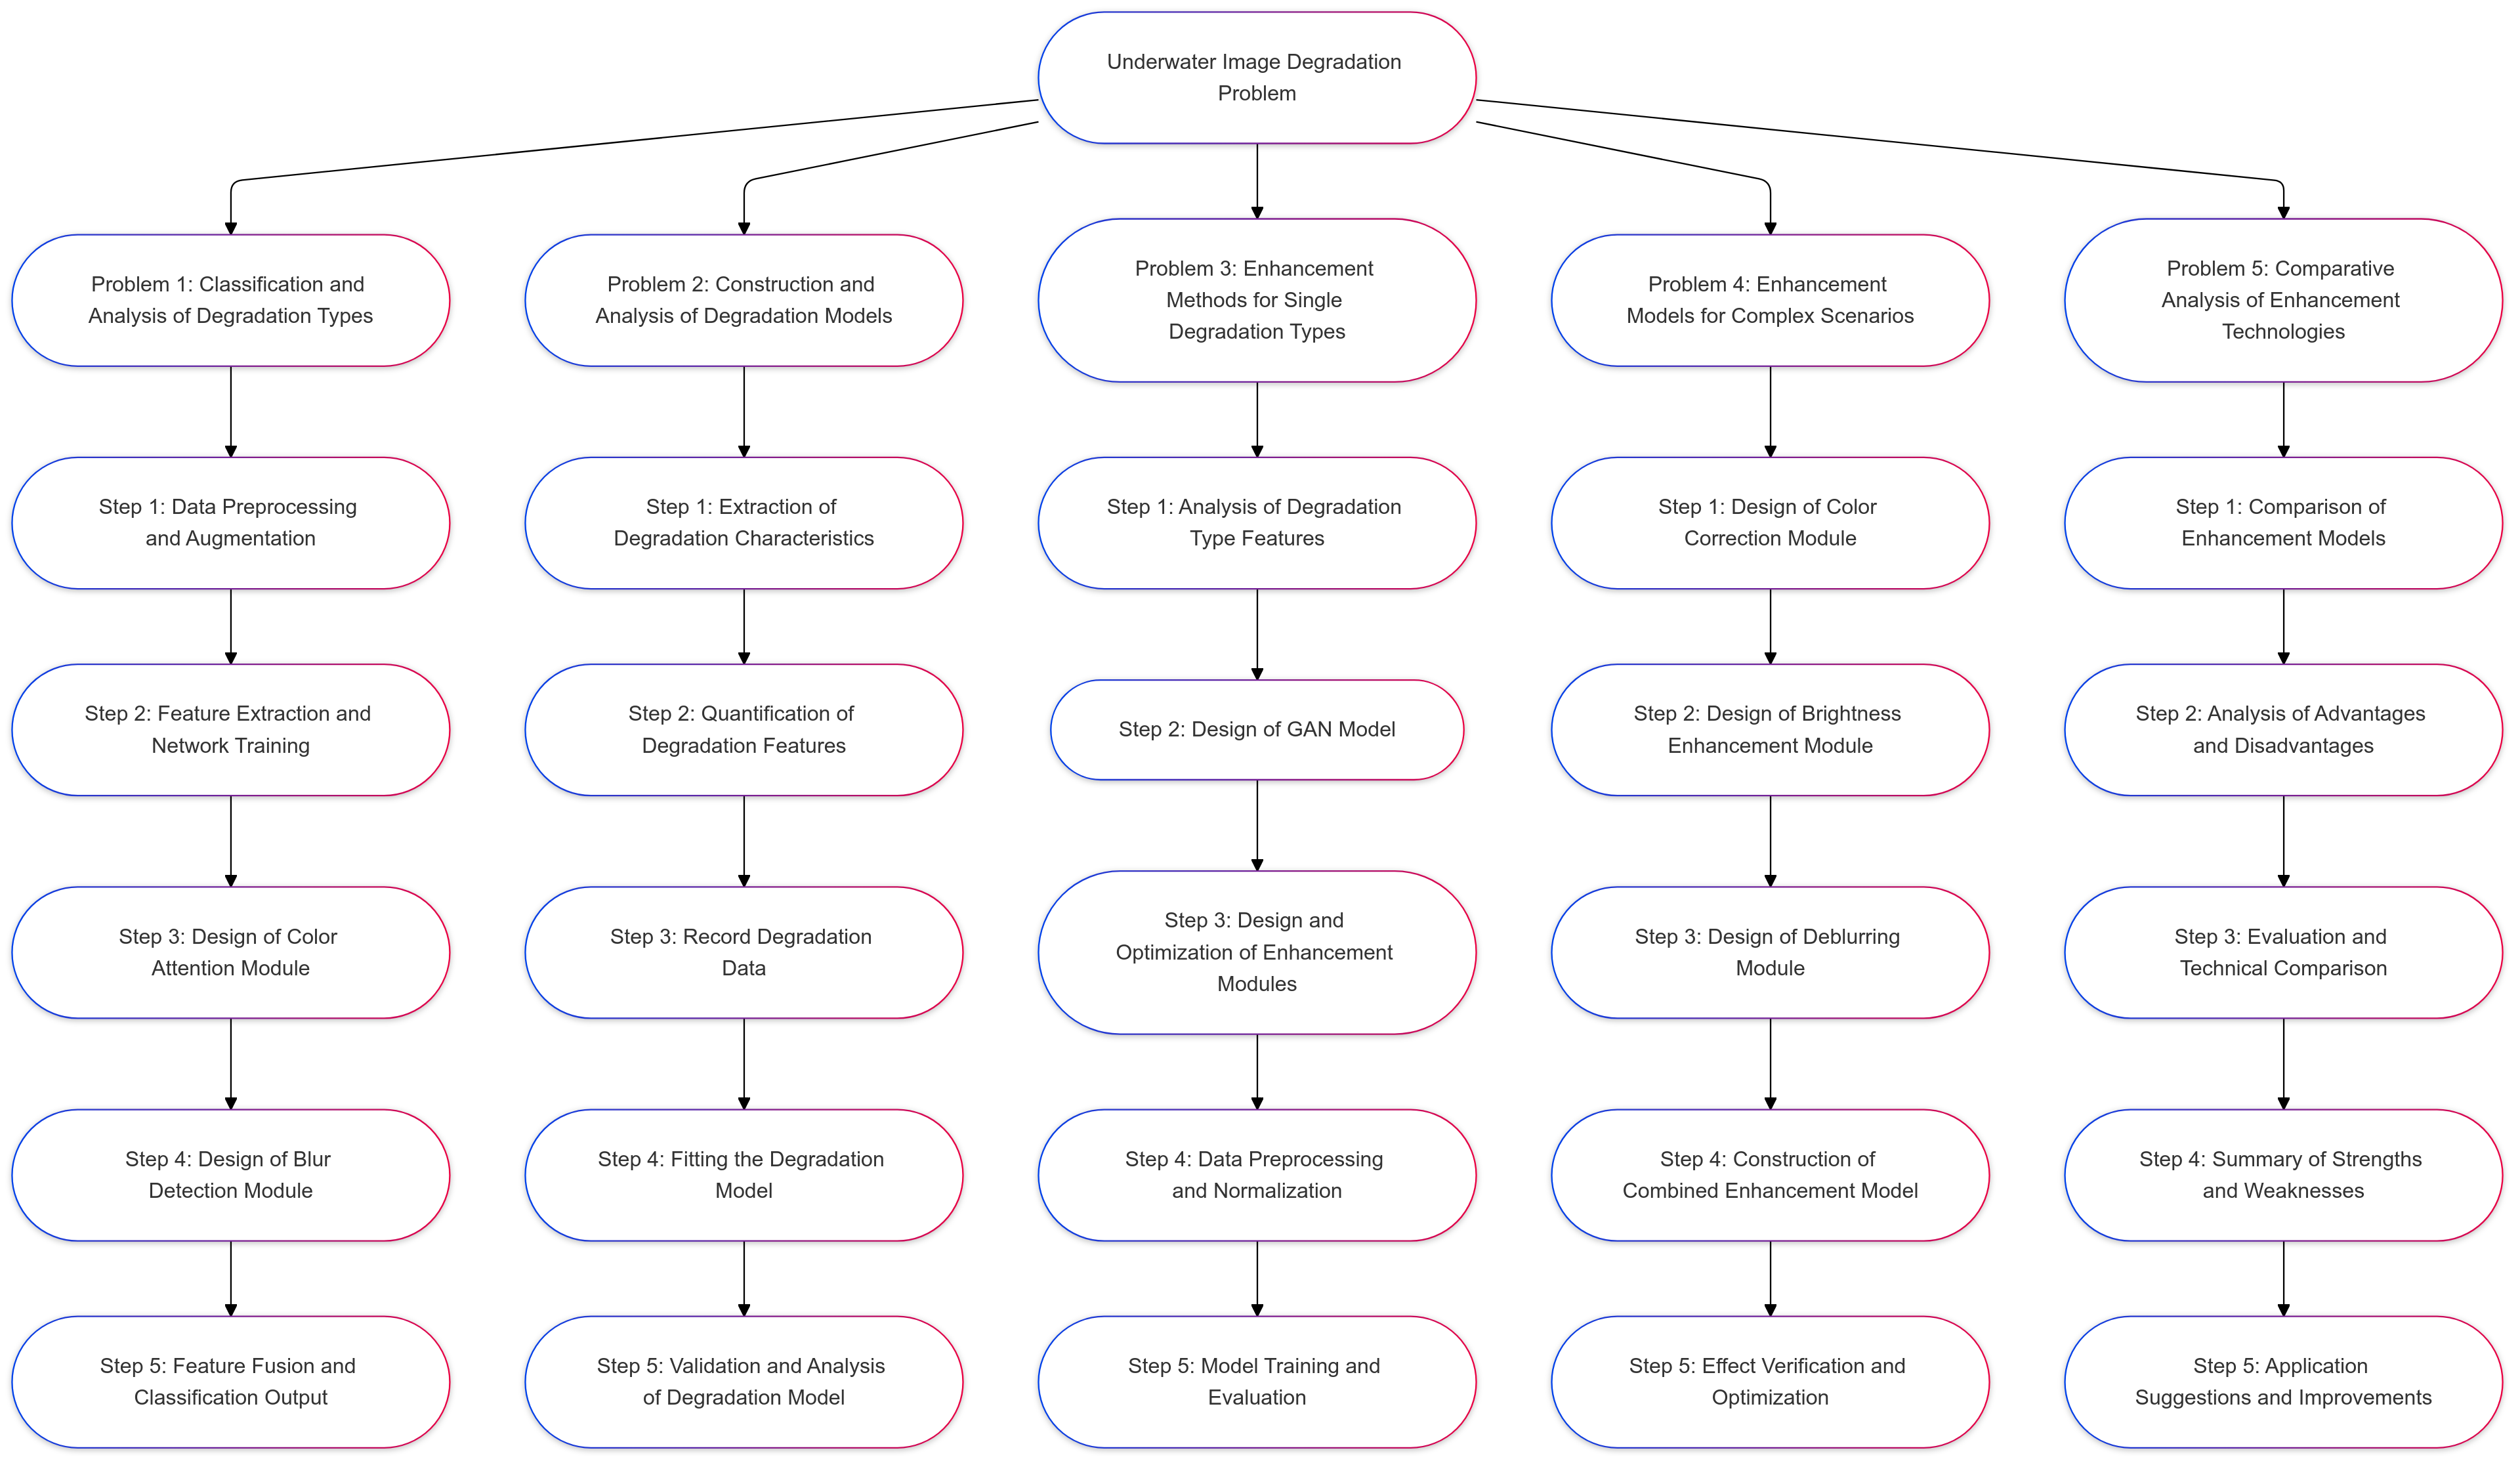
\includegraphics[width=\textwidth]{网络-总体流程图-2024-11-24-081146.png}
    \caption{General flow chart}
    \label{fig:enter-label}
\end{figure}












\subsection{分点讨论引用实例}
\subsubsection{分点方案1}

\begin{enumerate}
    \item \textbf{Adopt Comprehensive Models:} For real-world applications with multiple overlapping degradation types, comprehensive enhancement models should be prioritized. These models excel in addressing multifaceted degradation challenges, offering a more reliable and holistic solution compared to single-degradation approaches.
    \item \textbf{Refine Model Parameters:} Continuous refinement of the comprehensive model's parameters is essential to enhance its performance in varied environments. Adjusting factors like the relative contributions of color correction, brightness improvement, and sharpness enhancement can optimize results for specific degradation patterns.

\end{enumerate}

\subsubsection{分点方案2}
\begin{itemize}
\item \textbf{Powerful feature extraction capabilities:} Deep learning models can automatically extract features from images and adapt to complex underwater scenes. By training with large amounts of data, it is possible to learn degenerate patterns such as blur, color distortion, and low light.
Modern architectures such as convolutional neural networks (CNNS) can process underwater images with various degrees of degradation and have strong scene adaptability.
\item \textbf{data-driven optimization:} With the introduction of more diverse data, the model can be gradually improved, even to accommodate rare degradation scenarios.
\end{itemize}



\end{document} 